%! TEX program = xelatex

\documentclass{article}
\usepackage[a4paper, margin=3cm]{geometry}
\setlength{\parindent}{0pt}
\setlength{\parskip}{1em}
\usepackage{fontspec}
\setmainfont{Lato}

\usepackage{amsmath,amssymb,amsthm}
\usepackage{graphicx}
\usepackage{verbatim}
%\usepackage{pgfplots}
%\pgfplotsset{compat=1.16}

\title{}
\author{Mikael Myyrä}
\date{}

\begin{document}

\section*{1.}

Tämä on homogeeninen versio viime kerran tehtävä 3:sta hieman erilaisilla
reunaehdoilla. Nyt mukana on sekä Neumann- että Dirichlet-ehtoja.
Käytetään diskretointia
\[
  \frac{-u_{i,j-1} - u_{i-1,j} + 4u_{i,j} - u_{i+1,j} - u_{i,j+1}}{h^2} = 0.
\]
Keskeisdifferenssikaava Neumann-reunaehdoille on
\[
  \frac{u_{1,j} - 2u_{0,j} + u_{-1,j}}{2h} = 0
\]
alueen vasemmalla reunalla ja
\[
  \frac{u_{i,1} - 2u_{i,0} + u_{i,-1}}{2h} = 0
\]
alareunalla. Tähän tarvitaan haamupisteet $(i,-1)$ ja $(-1,j)$.
Laajentamalla laskenta-alue $([1, N] \times [1, N])$:stä
$([0, N] \times [0, N])$:n saadaan haamupisteiden vaikutus mukaan.

Matlab-koodi:

\verbatiminput{w4_1.m}

Lopputulos:

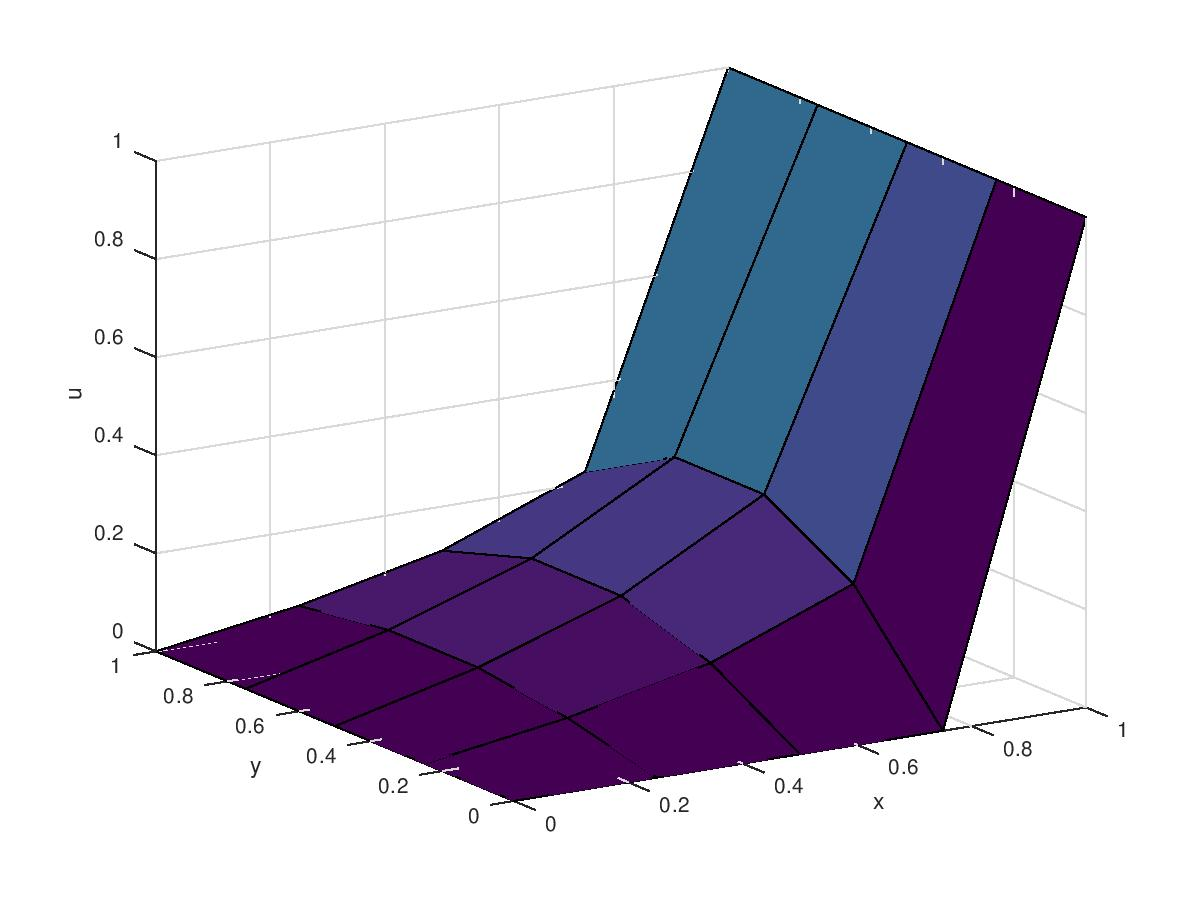
\includegraphics[width=350pt]{w4_1.jpg}

\newpage

\section*{2.}

Toteutin yhden ratkaisijan, johon voi parametrin arvolla määrätä,
käytetäänkö eksplisiittistä vai implisiittistä aika-askellusta.

Ratkaisijan koodi:

\verbatiminput{w4_heat.m}

Tämän tekemisessä paljon aikaa kului reunaehtojen ihmettelyyn ja erityisesti sen
huomaamiseen, että reunaehdon arvo piti kertoa $\alpha$:lla.

Seuraava koodi käyttää tätä ratkaisijaa tehtävään, jossa lähde on $f(x,y) =
3\sin(\pi x)\sin(\pi y)$, alkutila on $u(x,y,0) = \sin(3\pi x)\sin(3\pi y)$,
diffuusiokerroin $\alpha = 0.2$ ja reunaehdot $\frac{\partial u(0,y)}{\partial
\mathbf{n}} = \frac{\partial u(1,y)}{\partial \mathbf{n}} = 0$, $u(x,0) =
0.5\sin(\pi x)$ ja $u(x,1) = -0.5\sin(\pi x)$.  Ajassa edetään hetkeen 0.5 asti
200 askeleella.  Suoritusaikaa mitataan hilaväleillä $\frac{1}{10}$ ja
$\frac{1}{20}$ ja kuva piirretään näistä jälkimmäisellä.

\verbatiminput{w4_2.m}

Muutamalla kokeilulla hilavälillä $\frac{1}{10}$ kuluu prosessoriaikaa
eksplisiittisellä aika-askelluksella n. 0.40—0.45s ja implisiittisellä n.
1.0—1.1s.  Hilavälillä $\frac{1}{20}$ kuluu eksplisiittisellä n. 2.8—3.0s ja
implisiittisellä n. 7.1—7.3s.
Tällä pienellä otoksella implisiittinen menetelmä olisi karkeasti 2.5 kertaa hitaampi
kuin eksplisiittinen, mutta tämä ei varmasti ole lineaarinen suhde kun ratkaistavat
matriisit kasvavat suuremmiksi.

Eksplisiittisestä aika-askelluksesta huomasin kokeilemalla, että tässä käytetty
aika-askelen pituus on melko lähellä maksimia, jonka jälkeen menetelmä muuttuu
epästabiiliksi.

Kuva alkutilanteesta:

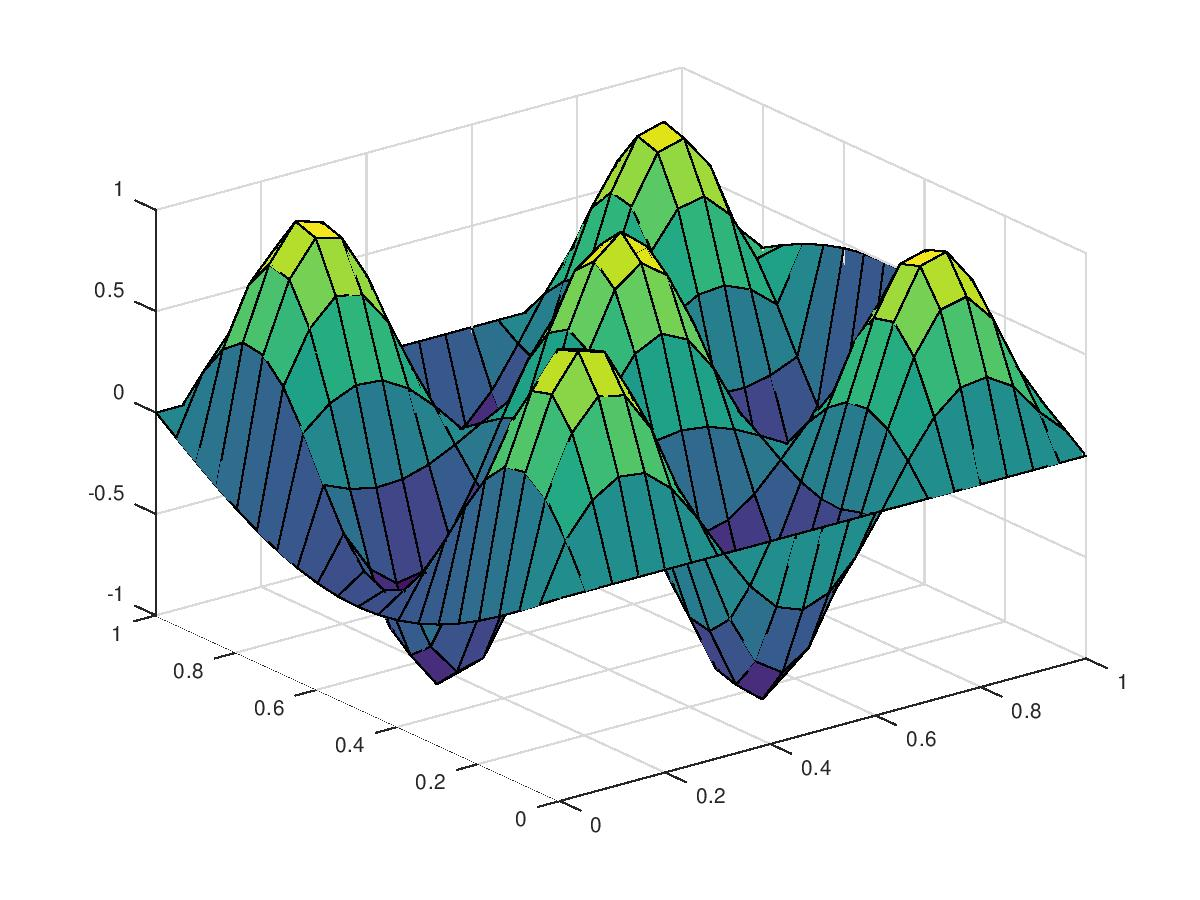
\includegraphics[width=350pt]{w4_2_start.jpg}

Ja aika-alueen lopussa:

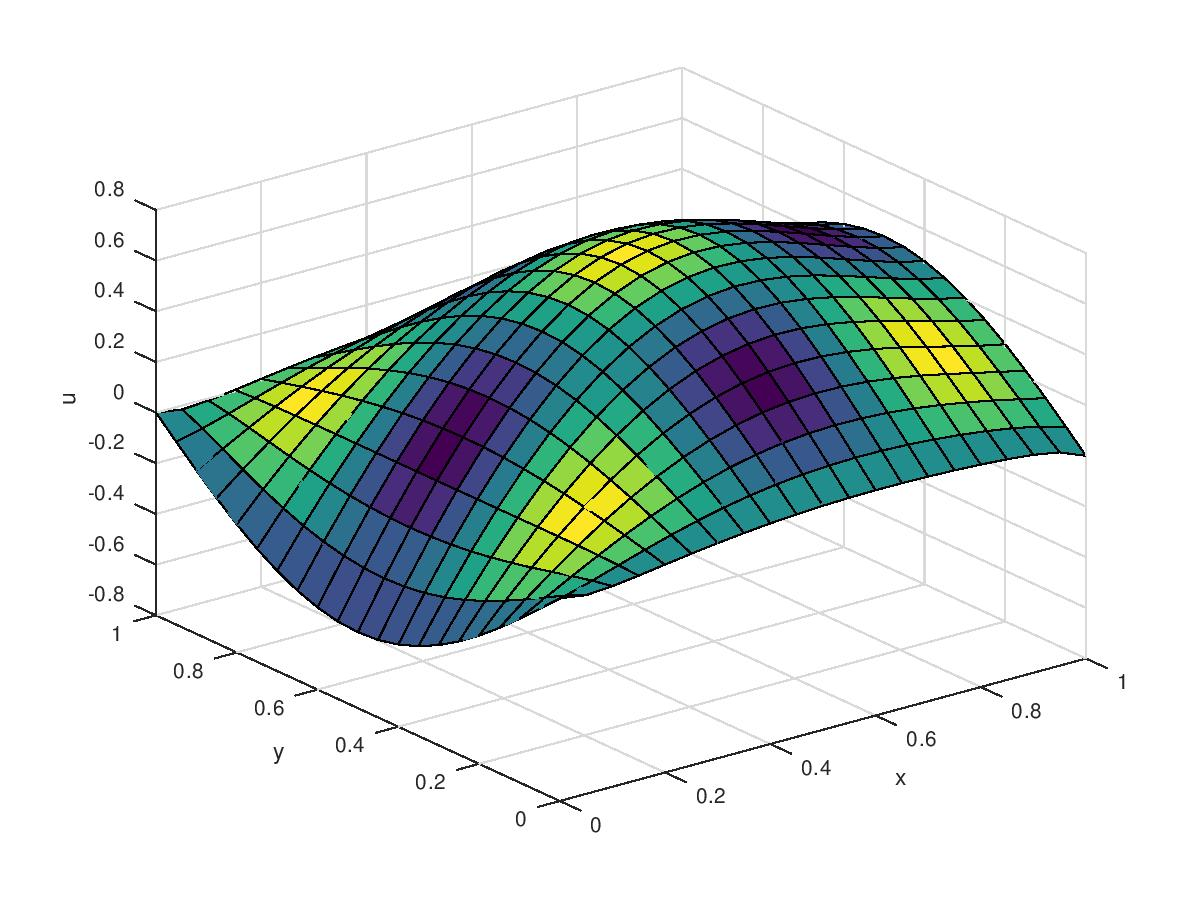
\includegraphics[width=350pt]{w4_2_end.jpg}

\newpage

\section*{3.}

Muotoilin edellisen tehtävän ratkaisijan niin, että tämä onnistuu
samalla funktiolla valitsemalla sopivat parametrit.

Tehtävä ei mainitse, mikä on alkutilanne. Tulkitsen niin, että voidaan aloittaa
(esimerkiksi) yläreunan matalammasta arvosta ja antaa lämmön tasaantua ajan kuluessa.

Matlab-koodi:

\verbatiminput{w4_3.m}

Tulos aika-alueen lopussa:

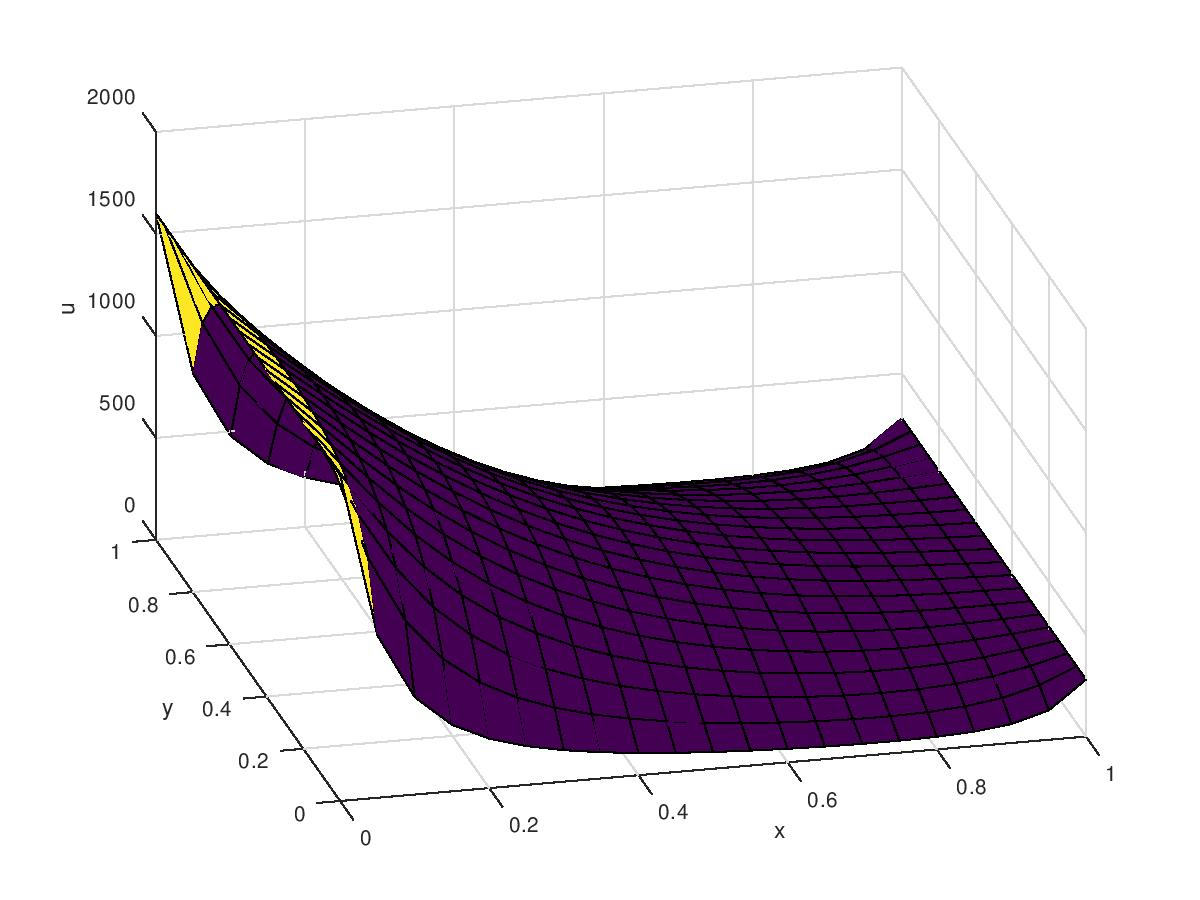
\includegraphics[width=350pt]{w4_3.jpg}

Etäisyyden yksikköä ei ole tässä määritelty; halutessaan välin (0, 1) voisi skaalata
vastaamaan todellista välimatkaa tutkittavien kerrosten välillä.

\newpage

\section*{4.}

\subsection*{(a)}

Lomakkeen lauseke on
\[
  T_{k+1} = T_k - \frac{\Delta t}{\Delta x} (u(T_k - T_{west}) + v(T_{north} - T_k))
\]
missä $T_{k}$ on lämpötila ajan hetkellä $k$, $\Delta t$ on aika-askel ja
$\Delta x$ on paikka-askel. Tekstistä ei selviä varmaksi, mitä $u$ ja $v$
ovat, mutta tulkitsen ne tuulen nopeuksiksi x- ja y-suunnissa.

Tämä näyttää eksplisiittisellä Euler-menetelmällä aikadiskretoidulta
homogeeniselta tehtävältä. Siirtämällä termejä saadaan
\[
  \frac{T_{k+1} - T_k}{\Delta t} + (u\frac{T_k - T_{west}}{\Delta x} + v\frac{T_{north} - T_k}{\Delta x}) = 0.
\]
Tässä ensimmäinen termi approksimoi aikaderivaatttaa $\frac{\partial T}{\partial t}$
ja toinen on sisätulo nopeusvektorista $\mathbf{w} = (u,v)$ ja lämpötilan
gradientin $\nabla T$ approksimaatiosta, joka on x-suunnassa takeneva
differenssi ja y-suunnassa etenevä differenssi.
Tämä sisätulo on suuntaisderivaatta $\frac{\partial T}{\partial \mathbf{w}}$.
Siis approksimoitava yhtälö on
\[
  \frac{\partial T}{\partial t} + \frac{\partial T}{\partial \mathbf{w}} = 0.
\]

\subsection*{(b)}

Differenssiapproksimaatiot on muotoiltu niin, että oikean ja alareunan arvoja
ei näy yhtälössä lain\-kaan, joten tulkitsen niin, että näillä reunoilla ei ole
myöskään reunaehtoja. Sen sijaan vasemman ja yläreunan arvot ovat mukana yhtälöissä,
joten niiden arvot täytyy olla annettu, ja ne toimivat Dirichlet-reunaehtoina.
Neumann-reunaehtoihin tarvittaisi ylimääräinen rivi laskentapisteitä.

\newpage
\section*{5.}

Jos tulkitsin edellisessä tehtävässä reunaehdot oikein, niin tässä tarvitaan
annettujen tietojen lisäksi reunaehto alueen vasempaan reunaan, missä $u > 0$.
Koska $v = 0$ ylä- ja alareunalla, niin reuna-arvoja ei siellä tarvita.
Epäilen hieman omia päätelmiäni, koska tehtävänannossa ei ole mainittu
reunaehtoja, mutta teen nyt ratkaisun tällä tulkinnalla. Valitsen reuna-arvoiksi
samat kuin niiden viereisissä pisteissä, eli 5.

$v$:n arvot ovat positiivisia, joten virtaus menee tässä ylöspäin, mikä on
vastakkainen suunta artikkelin tehtävään nähden. Lienee tarkoituksenmukaista
muuttaa derivaatta-approksimaatio takenevaksi differenssiksi myös y-suunnassa.
Saadaan paikkadiskretointi
\[
  \frac{\partial T}{\partial t} +
  \frac{1}{\Delta x}
  \begin{bmatrix}
    \,d_1 \\
    -u_2 & d_2 \\
       & -u_3 & d_3 \\
    -v_4 & & 0 & d_4 \\
       & -v_5 & & -u_5 & d_5 \\
       & & -v_6 & & -u_6 & d_6 \\
       & & & -v_7 & & 0 & d_7 \\
       & & & & -v_8 & & -u_8 & d_8 \\
       & & & & & -v_9 & & -u_9 & d_9 \,\\
  \end{bmatrix}
  \begin{bmatrix}
    \,T_1\, \\ T_2 \\ T_3 \\ T_4 \\ T_5 \\ T_6 \\ T_7 \\ T_8 \\ T_9
  \end{bmatrix}
  =
  \frac{1}{\Delta x}
  \begin{bmatrix}
    u_1 g_0 \\ 0 \\ 0 \\ u_4 g_4 \\ 0 \\ 0 \\ u_7 g_7 \\ 0 \\ 0
  \end{bmatrix}
\]
missä $g_0, g_4, g_7 = 5$ ovat reunaehdot alueen vasemmalla reunalla
ja $d_i$ on summa $u_i + v_i$.

Tehdään aikadiskretointi samalla tavoin kuin artikkelissa eli eksplisiittisesti,
\[
  \frac{T_{k+1} - T_k}{\Delta t} + AT_k = b
\]
\[
  T_{k+1} = T_k - \Delta t AT_k + \Delta t b.
\]

Hilavälin pituus on artikkelissa 100km ja aika-askel 3600s. Käytetään samoja arvoja.

Matlab-koodi:

\verbatiminput{w4_5.m}

Lopputulos:

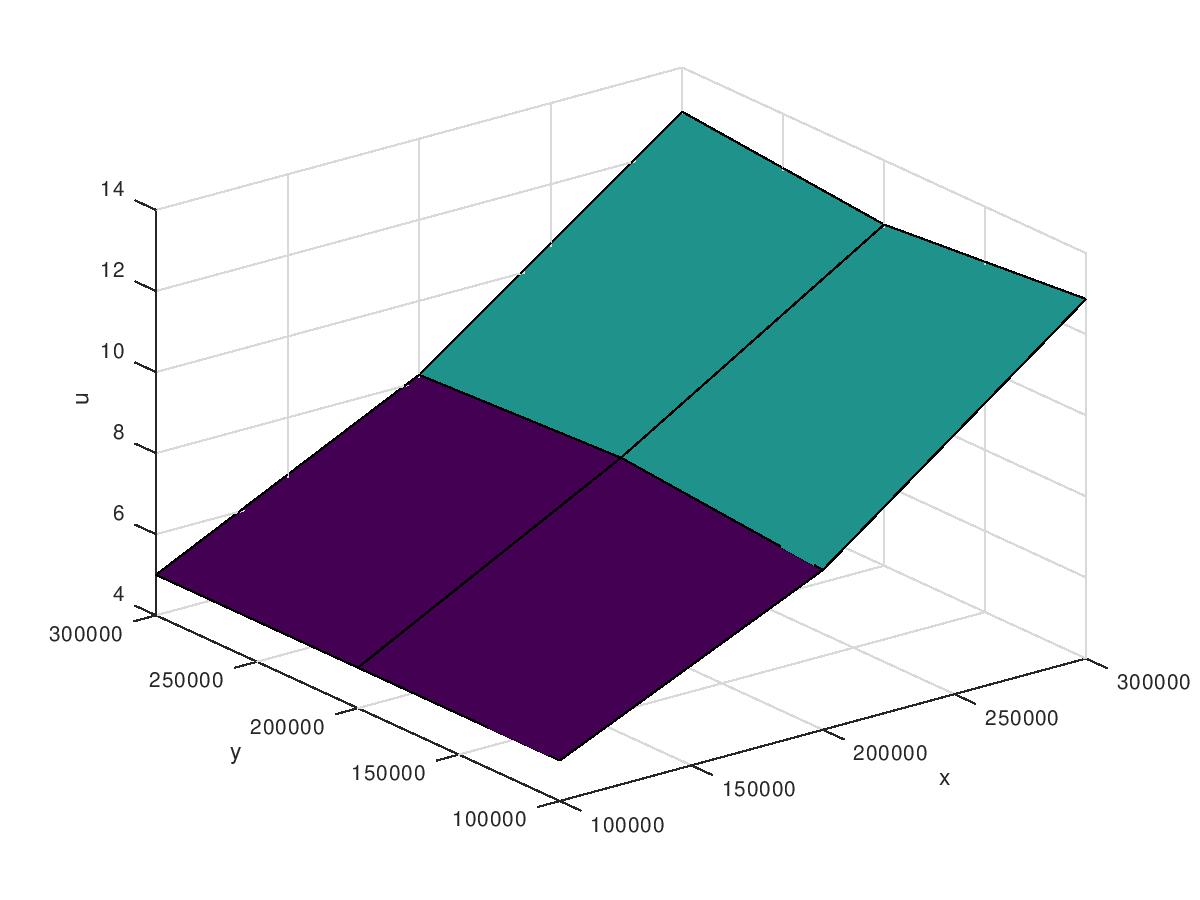
\includegraphics[width=350pt]{w4_5.jpg}

Lämpötila alueen oikeassa reunassa ja keskellä viileni hieman, ja viilenemisen
määrä vaihteli y-akselin suunnassa, mikä vaikuttaa uskottavalta tulokselta.

\end{document}
